\documentclass[10pt]{article}

\usepackage[a4paper,margin=1in]{geometry}
\usepackage{amsmath,amssymb,amsthm}
\usepackage{microtype}
\usepackage{graphicx}
\usepackage{booktabs}
\usepackage{enumitem}
\usepackage{xcolor}
\usepackage[hidelinks,colorlinks=true,linkcolor=black,citecolor=blue,urlcolor=blue]{hyperref}
\usepackage{titlesec}

\titleformat{\section}{\normalfont\large\bfseries}{\thesection}{0.6em}{}
\titleformat{\subsection}{\normalfont\bfseries}{\thesubsection}{0.6em}{}
\setlength{\parskip}{2pt}

\newcommand{\Rb}{\mathbb{R}}
\newcommand{\T}{^{\!\top}}
\newcommand{\Peff}{P_{\mathrm{eff}}}
\newcommand{\Qeff}{Q_{\mathrm{eff}}}
\newcommand{\Pbasis}{P_{\mathrm{basis}}}
\newcommand{\Qbasis}{Q_{\mathrm{basis}}}
\newcommand{\Pbases}{P_{\mathrm{bases}}}

\title{\textbf{Ortho-Hydra: Orthogonalised Experts for DiT LoRA}\\[2pt]
\large A structural fix for the MoE-LoRA cold-start deadlock}
\author{Seunghyun Ji\\\small\texttt{standingbehindnv@gmail.com}}
\date{April 2026}

\begin{document}
\maketitle

\begin{abstract}
LoRA fine-tuning of diffusion transformers (DiT) on multi-style data
suffers from \emph{style bleed}: a single low-rank residual cannot
hold several distinct artist fingerprints, so the optimiser settles on
their average. Mixture-of-experts LoRA (HydraLoRA-style) is the
obvious fix --- one shared down-projection, $E$ parallel up-heads, and a
router that picks a per-sample mixture --- but when every expert is
zero-initialised, the router receives identical gradient from each head
and stays at the uniform prior; experts evolve permutation-symmetrically
and the network trains as a single rank-$r$ LoRA paying $E\times$ the
cost. We present \textbf{Ortho-Hydra}, a re-parameterisation that
combines an OFT-style Cayley-orthogonal shared basis with
\textbf{per-expert disjoint output subspaces} carved from the top-$(Er)$
left singular vectors of the pretrained weight. Disjointness makes the
router's per-expert score genuinely different at step~$0$, so
specialisation has gradient signal before any expert has been trained.
The trained network bakes losslessly into a standard plain-LoRA
checkpoint (or a multi-head sibling for routing-aware loaders) because
the weight delta factors directly without SVD. We empirically confirm
the predicted deadlock against two HydraLoRA baselines on a matched
optimiser, dataset, and step budget: a zero-init shared-basis variant
and the original $\sigma\!=\!0.1$ Gaussian-jitter mitigation, neither
of which leaves the uniform routing prior in the first $1\text{k}$
steps, while disjoint slices begin de-uniformising within the first
few hundred. End-task generation quality on multi-style data is out
of scope here; we describe the construction, the cold-start mechanism,
and the failure modes the geometry fixes.
\end{abstract}

\section{Introduction}

Low-rank adaptation~\cite{hu2022lora} replaces a frozen weight $W_0
\in \Rb^{d_{\mathrm{out}}\times d_{\mathrm{in}}}$ with a residual
$y = W_0 x + s\,B A x$, where $A \in \Rb^{r\times d_{\mathrm{in}}}$ and
$B \in \Rb^{d_{\mathrm{out}}\times r}$ are trained and $s = \alpha/r$
is a scalar. For diffusion-transformer fine-tuning at $r \in [4,64]$
this is parameter- and storage-efficient and composes cleanly with the
ComfyUI-style ``weight-patch'' inference path, which is part of why it
has become the default adapter format for community LoRA distribution.

LoRA has two well-known weaknesses that compound on \emph{multi-style}
training data --- e.g.\ a single LoRA covering several artists. First,
the residual $BA$ can drift in directions that fight the pretrained
weight, so style adaptation also degrades anatomy or text rendering.
Second, with a single shared $(A,B)$ pair the optimiser's best rank-$r$
compromise across $K$ artists is the subspace that captures
\emph{common} structure --- the union becomes a blended average rather
than any individual fingerprint. The first weakness motivates
orthogonal fine-tuning~\cite{qiu2023oft,liu2024boft,wu2026psoft}, which
constrains the delta to a structurally orthogonal subspace; the second
motivates mixture-of-experts LoRA~\cite{tian2024hydralora}, which gives
the up-projection multiple heads under a learnt router so distinct
sample clusters can push different heads in different directions.

The two fixes solve different problems. They also \emph{compose
poorly} when stacked naively. We describe in
\S\ref{sec:method} an MoE-LoRA cold-start deadlock that arises when a
shared orthogonal basis is paired with multiple zero-initialised
expert heads, and a structural fix --- partitioning the top-$(Er)$
singular directions into disjoint per-expert slices --- that breaks the
deadlock at initialisation, before the router has trained at all.

\paragraph{Scope.} This is a focused methods report on the cold-start
mechanism. The construction is implemented and trains in our DiT
pipeline. We test the deadlock prediction against two shared-basis
HydraLoRA baselines on identical optimiser, dataset, and step budget
(Figure~\ref{fig:router-dynamics}): the predicted uniform-routing
plateau is directly observable in router entropy, and the original
$\sigma$-jitter mitigation does not escape it on the same budget.
End-task generation quality on multi-style data and sensitivity
ablations over $E$, $r$, and the balance-loss weight are out of scope
here.

\paragraph{Contributions.}
\begin{enumerate}[topsep=2pt,itemsep=0pt,leftmargin=1.2em]
\item We identify a cold-start deadlock specific to MoE-LoRA with a
shared orthogonal basis: every expert lives in the same rank-$r$
column span, so the router's per-expert score is an orthogonal-matrix
inner product that cannot be zero, the gates are near-equal at init,
and gradients to differentiate experts vanish.
\item We propose \emph{disjoint SVD-slice expert bases}: the top-$(Er)$
left singular vectors of $W_0$ are partitioned into $E$ orthonormal
slices, one per expert, rotated only \emph{within} their slice by a
per-expert Cayley matrix. Cross-expert orthogonality is preserved
through every gradient step.
\item We pair this with a \emph{layer-local} router that reads the
RMS-pooled rank-$r$ bottleneck activation (not the raw input, not the
text embedding), and explain why this aggregator is the only one of
three obvious choices that survives the long-sequence DC-cancellation
problem in DiT.
\item We show the trained network factors losslessly into a
plain-LoRA checkpoint --- $\Delta W$ is already rank-$r$, so no
post-hoc SVD is needed --- giving a deployable artefact for tooling
that does not understand routed adapters.
\end{enumerate}

\section{Background}
\label{sec:background}

\paragraph{LoRA.} Frozen $W_0$, residual $y = W_0 x + s\, B A x$,
$s = \alpha/r$. Standard practice~\cite{hu2022lora} initialises $B = 0$
so step~$0$ reproduces the base model exactly.

\paragraph{Orthogonal fine-tuning (OFT, BOFT, PSOFT).} Replace the free
delta $BA$ with a structurally-constrained one. OFT~\cite{qiu2023oft}
multiplies $W_0$ by a learned orthogonal matrix; BOFT~\cite{liu2024boft}
factors that matrix into a butterfly product for parameter
efficiency; PSOFT~\cite{wu2026psoft} restricts the rotation to the
\emph{principal subspace} of $W_0$ via a frozen SVD basis with a
Cayley-parameterised rotation inside that subspace. Cayley
parameterisation~\cite{lezcano2019cayley} guarantees orthogonality at
every step: for skew-symmetric $A = S - S\T$,
$R = (I-A)(I+A)^{-1}$ satisfies $R\T R = I$ exactly, with no
regularisation hyperparameter.

\paragraph{HydraLoRA.} The closest prior work~\cite{tian2024hydralora}
keeps the shared down-projection $A$ but replaces $B$ with $E$ parallel
up-heads $\{B_i\}_{i=1}^E$ and a router $g(\cdot) \in \Delta^{E-1}$
that emits a per-sample softmax gate. The effective up-projection
$B_{\mathrm{eff}}(x) = \sum_i g_i(x)\, B_i$ becomes sample-dependent.
With a Switch-Transformer~\cite{fedus2022switch} balance loss to keep
all experts alive, this gives distinct sample clusters room to push
different heads in different directions.

\paragraph{Soft expert-specialisation regularisers.}
A separate line of work~\cite{guo2025advancing} attacks expert
overlap in MoE \emph{post-training} from the loss side rather than
the architecture: an output-orthogonality term penalising inner
products between selected experts' per-token outputs and a
routing-variance term encouraging decisive gates, both stacked on
the standard auxiliary balance loss. The motivating regime is a
pretrained MoE whose experts already differ but whose router is
being driven back toward uniformity by the balance objective during
fine-tuning. Soft regularisation and structural reparameterisation
attack the overlap problem from different sides; we return to the
comparison once the construction is on the table.

\paragraph{The cold-start deadlock.} HydraLoRA initialises every $B_i$
to zero so the residual is zero at step~$0$ (LoRA-safe). Under a
near-uniform router every expert receives \emph{identical} gradient,
and the experts evolve permutation-symmetrically: they stay identical
forever, the router never gets a differentiating signal, and the
network trains as a single rank-$r$ LoRA averaged over $E$ heads. The
original mitigation is \emph{expert warm-up}: for the first
$\rho \cdot N_{\mathrm{steps}}$ steps, only a randomly-chosen expert
per module receives gradient at each step, breaking the symmetry by
schedule. This works, but it is fragile to schedule choices and
provides no signal to the router until $B_i$ have drifted apart.

\section{Method: Ortho-Hydra}
\label{sec:method}

\subsection{Architecture}

For each adapted Linear $W_0 \in \Rb^{d_{\mathrm{out}}\times d_{\mathrm{in}}}$
we store
\begin{center}
\small
\begin{tabular}{@{}lll@{}}
\toprule
Component & Shape & Trainable? \\
\midrule
$\Qbasis$ & $(r,\, d_{\mathrm{in}})$ & frozen buffer (shared) \\
$\Pbases$ & $(E,\, d_{\mathrm{out}},\, r)$ & frozen buffer (per-expert disjoint) \\
$S_q$ & $(r,\, r)$ & yes, shared \\
$S_p$ & $(E,\, r,\, r)$ & yes, per-expert \\
$\lambda$ & $(1,\, r)$ & yes, shared \\
$\theta_{\mathrm{router}}$ & $\Rb^{(r+d_\sigma)\times E} \times \Rb^E$ & yes, layer-local \\
\bottomrule
\end{tabular}
\end{center}

Compute the thin SVD of $W_0$ via randomised
SVD~\cite{halko2011randomized},
$W_0 \approx U\Sigma V\T$, with $U \in \Rb^{d_{\mathrm{out}}\times q}$
and $V \in \Rb^{d_{\mathrm{in}}\times q}$ at $q = Er + 6$. Set
\[
\Qbasis \leftarrow V_{:,1:r}\T,
\qquad
\Pbases[e] \leftarrow U_{:,\,(e-1)r+1:\,er}
\;\;\text{for}\;\; e=1,\dots,E.
\]
$\Qbasis$ has orthonormal rows, and the $\Pbases[e]$ are
\emph{mutually orthonormal} slices of $U$:
$\Pbases[i]\T \Pbases[j] = \mathbf{0}$ for $i \neq j$ and $= I_r$ for
$i=j$. This is the load-bearing geometric property; we return to it in
\S\ref{sec:deadlock-fix}.

The trainable rotations are skew-symmetric seeds. Given $S_q$ and
$S_p[e]$, define $A_q = S_q - S_q\T$ and $A_p[e] = S_p[e] - S_p[e]\T$,
and form Cayley orthogonal matrices
\[
R_q = (I - A_q)(I + A_q)^{-1},
\qquad
R_p[e] = (I - A_p[e])(I + A_p[e])^{-1}.
\]
We compute the inverse with \texttt{torch.linalg.solve} rather than a
Neumann truncation~\cite{wu2026psoft}: at $r \leq 64$ the cost is
negligible and the solve is unconditionally correct, whereas a
$K$-term Neumann series silently diverges when $\lVert A\rVert > 1$ and
breaks orthogonality without any signal in the loss.

The effective bases
$\Qeff = R_q \Qbasis$ (rows orthonormal, shared)
and $\Peff[e] = \Pbases[e]\, R_p[e]$ (columns orthonormal within
slice $e$) preserve cross-expert orthogonality exactly through
training: $\Peff[i]\T \Peff[j] = R_p[i]\T\, \Pbases[i]\T\, \Pbases[j]\,
R_p[j] = \mathbf{0}$ for $i \neq j$, and $= R_p[i]\T R_p[j]$
otherwise.

\subsection{Forward and routing}

For input $x \in \Rb^{B\times L\times d_{\mathrm{in}}}$,
\begin{align*}
\ell &= x\,\Qeff\T \in \Rb^{B\times L\times r}, \\
g    &= \mathrm{softmax}\bigl(\theta_{\mathrm{router}}\bigl[\mathrm{rmspool}_L(\ell)\,\big\Vert\,\phi(\sigma)\bigr]\bigr) \in \Delta^{E-1}, \\
\ell &\leftarrow \ell\,\odot\,\lambda, \\
P_{\mathrm{combined}}(b) &= \sum_{e=1}^{E} g_{b,e}\,\Peff[e] \quad\in\Rb^{d_{\mathrm{out}}\times r}, \\
y    &= W_0 x + s\,P_{\mathrm{combined}}\,\ell.
\end{align*}
Here $\mathrm{rmspool}_L(\ell)_j = \sqrt{(1/L)\sum_\ell \ell_{\cdot,\ell,j}^2}$
is RMS pool over the sequence dimension, $\phi(\sigma)$ are
sinusoidal features of the diffusion noise level (optional, zero-init
columns in the router so step-$0$ behaviour matches the no-$\sigma$
case).

\paragraph{Why RMS over rank-$r$, not the obvious alternatives.}
Pooling over a $\sim$$4096$-token DiT sequence breaks zero-mean
features under mean-pooling: per-channel std after the mean is
$\sigma_x / \sqrt{L} \approx 0.008$, so the pooled vector is
near-identical across samples and the router sees effectively constant
input. Pooling \emph{after} the rank-$r$ bottleneck rather than over
raw $d_{\mathrm{in}}$-wide activations also matters --- DiT layer
inputs have heavy DC-bias outlier channels (peak/mean ratios in the
$80$--$96\times$ range) that saturate softmax in bf16 under max
pool, and the rank-$r$ space is bounded by
$\lVert\Qbasis\rVert\cdot\lVert x\rVert$ with no such outliers. RMS,
unlike mean, does not cancel zero-mean signals by $\sqrt{L}$ because
signs square to positive before averaging. Of three pool/space
combinations we tried, this is the only one whose router weight norm
moves from initialisation; the other two left the router
indistinguishable from random init at end of training.

\subsection{Why disjoint slices break the deadlock}
\label{sec:deadlock-fix}

The router's per-expert score before softmax can be written, ignoring
the $\sigma$-feature columns, as
\[
\mathrm{score}_e \;=\; w_e\T \,\mathrm{rmspool}_L\bigl(x\,\Qeff\T\bigr)
\]
with $w_e \in \Rb^r$ a slice of the router weight. At init $\lambda =
0$, so the residual is zero and the gradient into $w_e$ comes from
the chain rule through $\Peff[e]$ when $\lambda$ takes its first
non-zero step. The relative magnitudes of $w_e$'s gradients are
governed, to first order, by the Gram matrix
$\Peff[i]\T \Peff[j]$:

\begin{itemize}[topsep=2pt,itemsep=0pt,leftmargin=1.2em]
\item \textbf{Shared basis (the bad case).} If every expert uses the
same $\Pbasis$, then $\Peff[i]\T \Peff[j] = R_p[i]\T R_p[j]$ is an
$r\times r$ orthogonal matrix --- it cannot be zero, and at zero-init
$S_p$ it is the identity. Every expert produces the same per-token
output direction; gradients into the $w_e$ are near-identical;
softmax gates stay near $1/E$; gradient into $S_p[e]$ is the same for
every $e$; experts evolve permutation-symmetrically. This is the
deadlock.

\item \textbf{Disjoint slices (our case).} If $\Pbases[i]\T
\Pbases[j] = \mathbf{0}$ for $i \neq j$, then so is $\Peff[i]\T
\Peff[j]$ for every value of $S_p$. Each expert writes into a
\emph{distinct} output subspace; the per-expert components of the
upstream gradient are orthogonal in $\Rb^{d_{\mathrm{out}}}$, so the
projections onto each $w_e$ are genuinely different. The router has
signal before any expert has trained.
\end{itemize}

This is a structural deadlock breaker, not a schedule, and it
operates one level below loss-side specialisation
regularisers~\cite{guo2025advancing}: at zero-init $S_p$ a per-token
output-orthogonality penalty has identical operands across experts
and a routing-variance penalty operates on identical logits, so both
regulariser gradients are themselves permutation-symmetric in the
expert index and cannot break the symmetry they share. The geometric
construction makes per-expert gradient direction non-degenerate from
step~$0$, which is what such regularisers cannot do for themselves.
It does not replace the Switch-Transformer balance loss --- that
still does its own job, keeping all experts alive against the
tendency of a sharp router to collapse onto one --- but it removes
the bootstrapping problem the balance loss alone cannot solve.

\paragraph{When disjointness is impossible.}
The construction requires
$\min(d_{\mathrm{out}}, d_{\mathrm{in}}) \geq Er$. For DiT-scale
attention and MLP weights with $d \in \{1024, 3072, 4096\}$ and our
default $E=4$, this is satisfied at every rank we have used
($r \leq 64$). On narrow projections that would violate the inequality
the implementation falls back to a shared-basis $\Pbases$ replicated
across experts (with a runtime warning); in that fallback the only
symmetry-breaker is the original expert warm-up schedule, and
running with warm-up disabled is unsafe.

\subsection{Lossless bake-down to plain LoRA}

The trained delta is
\[
\Delta W(b)
\;=\; \sum_{e=1}^{E} g_{b,e} \,\Peff[e]\,\mathrm{diag}(\lambda)\,\Qeff
\;\;\in\;\;\Rb^{d_{\mathrm{out}}\times d_{\mathrm{in}}}.
\]
The per-sample $\Delta W(b)$ has rank at most $r$ (sum of $E$
rank-$r$ outer products lying in disjoint output subspaces but a
shared $r$-dimensional input subspace via $\Qeff$). At save time we
average gates across the population (uniform prior approximation,
$\bar g_e = 1/E$) and write
\[
\bar\Delta W = \tfrac{1}{E}\!\sum_{e} \Peff[e]\,\mathrm{diag}(\lambda)\,\Qeff
= \bar P_{\mathrm{eff}}\,\mathrm{diag}(\lambda)\,\Qeff
\]
which is exactly rank-$r$ and factors directly without SVD into
$(\mathrm{lora\_up}, \mathrm{lora\_down})$ via a square-root split of
$\lambda$. We ship two files side by side: a plain-LoRA checkpoint
that any LoRA-aware loader can consume (lossy: routing collapsed to
the uniform prior), and a multi-head sibling that preserves the
trained gates for a router-aware custom node. The bake-down is
arithmetically exact; nothing is left on the table.

\section{Experiments}
\label{sec:experiments}

\begin{figure}[t]
\centering
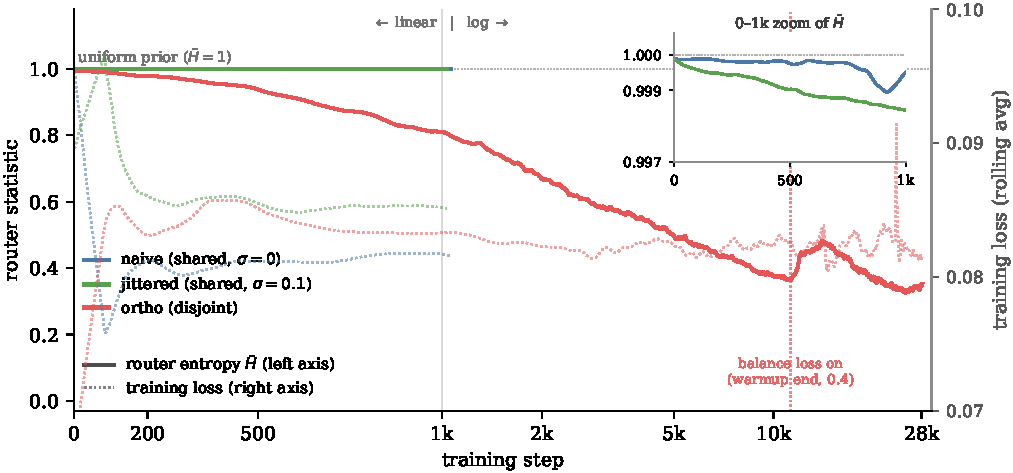
\includegraphics[width=\linewidth]{router_dynamics.pdf}
\caption{Cold-start router dynamics across three HydraLoRA variants
($E\!=\!12$, balance-loss weight $5\!\times\!10^{-7}$ with warmup
ratio $0.4$, AdamW, identical dataset and optimiser schedule). Solid:
mean normalised router entropy $\bar H$ (left axis); dotted: training
loss (right axis), zoomed to $[0.07, 0.10]$ as a proof-of-life signal.
\emph{Naive} (shared basis, zero-init experts) and \emph{jittered}
(shared basis $+$ $\sigma\!=\!0.1$ Gaussian on $B_i$, the original
HydraLoRA mitigation~\cite{tian2024hydralora}) stay pinned at
$\bar H\!\approx\!1$ for the full $1\text{k}$ steps we ran them;
\emph{ortho} (disjoint slices) has left the uniform prior by step
$\sim\!200$ and converges to $\bar H\!\approx\!0.35$ over $28\text{k}$
steps. Inset: $0$--$1\text{k}$ window magnified to
$\bar H\!\in\![0.997, 1.0006]$ --- jitter buys only modest extra drift
over naive, so the deadlock is not a slow-training artefact. The
vertical at step $11266$ marks the balance-loss weight flipping on
($0.4\!\cdot\!28164$ max steps); the small entropy bump in ortho
around that step is the load-balance penalty pulling a specialised
router back toward uniform. Training loss on the right axis confirms
all three variants reach the same $\sim\!0.08$ band; the gap between
them is entirely in routing, not optimisation. \emph{Caveat:} ortho
ran at $r\!=\!48$ vs.\ $r\!=\!32$ for the baselines, but the
$\bar H$ gap is too large for a $1.5\!\times$ rank difference to
explain (and more rank does not help shared-basis routing). The
naive and jittered runs were stopped at $1\text{k}$ steps once the
plateau at $\bar H\!\approx\!1$ was unambiguous.}
\label{fig:router-dynamics}
\end{figure}

\paragraph{Base model.}
We adapt \emph{anima-preview3-base}~\cite{anima2026}, a $28$-block,
$2048$-channel DiT ($16$ heads of dim $128$ each, MLP ratio $4$)
trained with a flow-matching velocity-field objective on multi-style
anime data; text conditioning is a frozen Qwen3-0.6B base encoder,
and the latent codec is the qwen-image VAE. All three modules are
held frozen through training; only the LoRA / MoE adapter is updated.
The bf16 DiT checkpoint is ${\sim}\,4.2$\,GB.

\paragraph{Data.}
The training set is ${\sim}\,2.4\text{k}$ images covering several
artist styles, each with a free-form caption. We use masked loss
with masks merged from a SAM3 pass and a manga-text-detector pass
(text bubbles excluded from the loss). Latents are pre-cached via
the VAE and text outputs via the Qwen3 encoder, and the DiT is
loaded only after caching to free VRAM. Constant-token bucketing
rounds each sample to ${\sim}\,4096$ latent tokens with zero-padding,
giving \texttt{torch.compile} a single static shape across aspect
ratios.

\paragraph{Optimiser and schedule.}
AdamW (fused) at $\mathrm{lr}\!=\!2\!\times\!10^{-5}$, constant
schedule, no warmup. bf16 mixed precision; flow shift $1.0$;
sigmoid timestep sampling; caption dropout $0.1$; T-LoRA timestep
masking enabled on every variant. Batch size $1$ per step at
constant-token-budget $4096$. The full ortho run is $28164$ steps
($12$ epochs over the dataset); shared-basis baselines are stopped
at $1\text{k}$ steps once the plateau at $\bar H\!\approx\!1$ is
unambiguous.

\paragraph{Adapter configuration.}
HydraLoRA is applied only to the two MLP linears
(\texttt{layer1}\,/\,\texttt{layer2}) of every DiT block ($28\!\times\!2 = 56$
adapted Linears in total) at $E\!=\!12$ experts and $\alpha\!=\!32$.
The router is layer-local with $4$-bucket sigma features (a sinusoidal
encoding of the diffusion noise level fed alongside the RMS-pooled
rank-$r$ activation), and its learning rate is scaled $10\!\times$
above the adapter LR. The Switch-Transformer~\cite{fedus2022switch}
balance loss has weight $5\!\times\!10^{-7}$ with warmup ratio $0.4$
(turn-on at step $11266 = 0.4\!\cdot\!28164$) and a per-bucket
coefficient of $0.3$ to keep each sigma-bucket's expert distribution
near-uniform. Variant-specific knobs:
\begin{itemize}[topsep=2pt,itemsep=0pt,leftmargin=1.2em]
\item \emph{naive}: shared-basis HydraLoRA, $r\!=\!32$, $B_i\!=\!0$,
no symmetry-breaker.
\item \emph{jittered}: shared-basis HydraLoRA, $r\!=\!32$, $B_i\!\sim\!\mathcal{N}(0,
0.1^2)$ --- the original HydraLoRA mitigation~\cite{tian2024hydralora}.
\item \emph{ortho}: this paper's construction with disjoint SVD-slice
expert bases, $r\!=\!48$. The $r$ mismatch with the baselines is a
wall-clock concession (the cold-start signal saturates by $\sim$$200$
steps and a rank-matched repeat seemed unlikely to change the
conclusion); see the figure caption.
\end{itemize}

\paragraph{Metrics.}
\emph{Mean normalised router entropy} $\bar H \in [0,\,1]$: per-Linear
softmax entropy divided by $\log E$ and averaged across the $56$
routed Linears, so $\bar H\!=\!1$ at the uniform prior and $\bar H\!=\!0$
at one-hot routing. \emph{Top1$-$top2 margin}: $g_{(1)}-g_{(2)}$
averaged over batch and routed Linears, a complementary
``decisiveness'' view that survives soft-routing where entropy moves
slowly. \emph{Training loss}: the standard flow-matching velocity MSE
(masked, as configured for training).

\paragraph{Results.}
Figure~\ref{fig:router-dynamics} shows the cold-start router dynamics
across the three variants. The two shared-basis runs stay pinned at
the uniform prior $\bar H\!\approx\!1$ for the full $1\text{k}$ steps
we ran them --- $\bar H$ moves by $<\!0.005$ and the top1$-$top2
margin by $<\!0.005$ --- while ortho has already left
$\bar H\!\approx\!0.81$ by step $1\text{k}$ and converges to
$\bar H\!\approx\!0.35$ over $28\text{k}$ steps, all twelve experts
alive at end. Training loss is essentially identical across variants
($\sim\!0.08$ end-of-run band, dotted right axis); the gap is in
routing, not optimisation. The de-uniformisation in ortho is also
clearly \emph{gradual} over the first ${\sim}\,2\text{k}$ steps rather
than instantaneous, because the router gradient is gated by
$\lambda$ having left zero --- so the deadlock claim is about
gradient \emph{direction} (the per-expert score is non-degenerate
from the start) rather than gradient \emph{magnitude} (initially
small, growing with $\lambda$). That the jittered baseline barely
outperforms naive is the single strongest observation: even an
aggressive $\sigma\!=\!0.1$ Gaussian on $B_i$, which fully randomises
the up-projection, cannot break the shared-basis deadlock at the
rate disjoint slices do.

\section{Discussion and limitations}

\paragraph{Subspace restriction is real.}
$\Delta W(b)$ is constrained to live in
$\mathrm{colspace}(\Pbases) \subseteq \mathrm{top}\text{-}(Er)$ left
singular vectors of $W_0$. For NLP fine-tuning this is a feature ---
the model already knows the domain and the delta nudges it
\emph{within} the domain~\cite{wu2026psoft}. For creative
fine-tuning of a diffusion model the assumption is shakier: a new
character or art style might require a $\Delta W$ component
\emph{outside} the principal subspace. We accept this trade; whether
the lost expressiveness matters for the multi-style fine-tuning
regime that motivated the construction is an empirical question we
do not answer here.

\paragraph{Disjointness is a strong constraint.}
We have argued that disjoint slices break the cold-start deadlock,
but we have not argued that disjoint slices are \emph{optimal} ---
only that they are sufficient and computable from the pretrained
weight without any training data. Other choices (Hadamard, structured
random) would also satisfy the inner-product condition. The SVD
choice is motivated by the same intuition as PSOFT: the top-$(Er)$
singular directions are where the pretrained weight already spends
its capacity, so an adapter delta that lives in those directions is
the most likely to be useful. This is a hypothesis, not a result.

\paragraph{Why $\sigma$-jitter is brittle in practice.}
The Gaussian-noise mitigation has two failure modes that the
disjoint-slice construction sidesteps by having no analogous knob.
First, the noise is loss-agnostic: it perturbs each $B_i$ in random
directions in $\Rb^{d_{\mathrm{out}}}$, but those directions are
generically unaligned with the directions in which the multi-style
data wants to push different experts, so a shared-basis gradient ---
identical across experts up to whatever residual asymmetry the noise
created --- ironed out our $\sigma\!=\!0.1$ separation well before
the balance loss had even turned on. The 1k-step jittered run in
Figure~\ref{fig:router-dynamics} executed entirely inside the
balance-loss warmup region (turn-on at step $11266 = 0.4\!\cdot\!N$),
yet $\bar H$ moved by $<\!0.005$ over that window: shared-basis
dynamics flatten the noise on their own, with no help from the load
balancer. Second --- a hypothetical extension of the failure mode
once the run is long enough --- the $\sigma$-jitter window has an
upper bound at the balance-loss turn-on step $\rho_b\!\cdot\!N$:
whatever tentative per-expert separation has accumulated by then is
pulled back toward uniform by the load-balance penalty, so $\sigma$
must be aggressive enough for stable specialisation to emerge from
shared-basis flattening within $\rho_b\!\cdot\!N$ steps but not so
aggressive that the random initial residual destabilises early
training. This is a fragile two-knob region $(\sigma, \rho_b)$ where
neither knob has a principled setting --- they are tuned by the same
criterion (router entropy) they are meant to fix. The structural fix
has neither knob: cross-expert orthogonality holds at step~$0$ by
construction and survives every gradient step thereafter, so the
balance-loss schedule and the noise scale are both irrelevant to
whether the router de-uniformises.

\paragraph{What the cold-start experiment establishes.}
Disjoint output subspaces give the router non-degenerate gradient at
initialisation; Figure~\ref{fig:router-dynamics} tests that mechanism
claim at its strongest resolution. The shared-basis deadlock is
directly observable in router entropy, and even the original
HydraLoRA $\sigma$-jitter mitigation does not escape it on a matched
step budget --- so the deadlock is not a slow-training artefact, and
not a missing-noise artefact either: it is a property of shared-basis
gradient geometry, and the structural fix removes it. What the
experiment does not test, and we leave for future work: (i)~generated-image
quality on multi-style fine-tuning, (ii)~sensitivity to $E$, $r$, and
the balance-loss weight, and (iii)~end-of-training comparisons at
matched rank (the baselines were $r\!=\!32$ vs.\ $r\!=\!48$ for ortho;
the cold-start signal saturates by $\sim\!200$ steps so a rank-matched
repeat seemed unlikely to change the routing conclusion). Whether
disjoint slices also improve end-task quality on multi-style data
is open.

\paragraph{Soft specialisation regularisers vs.\ structural orthogonality.}
A complementary line of work~\cite{guo2025advancing} attacks the
MoE specialisation--uniformity tension with loss-side regularisers:
an output-orthogonality term on selected experts' per-token outputs
($\mathcal{L}_o = \sum_{i,j\neq k} \lVert \langle \tilde x_{ij}, \tilde
x_{ik}\rangle / (\langle \tilde x_{ik}, \tilde x_{ik}\rangle + \epsilon)
\cdot \tilde x_{ik}\rVert^2$, with $\tilde x_{ij} = x_i\,\theta_{E_j}\,
\mathbb{1}_{\{s_{ij}>0\}}$) and a routing-variance term that rewards
decisive gates ($\mathcal{L}_v = -\sum_{i,j}(s_{ij} - \bar s_j)^2/n$),
designed to coexist with a standard auxiliary balance loss without
sacrificing $\mathrm{MaxVio}$. These regularisers report consistent
gains on \emph{pretrained} MoE LLMs in post-training, where experts
already differ non-trivially and the failure mode is regression
\emph{toward} uniformity under aux-loss pressure. The cold-start
regime that motivates Ortho-Hydra is different: experts are freshly
initialised ($S_p\!=\!0$, $\lambda\!=\!0$) and the router is at the
uniform prior, so a per-token output-orthogonality loss operates on
$E$ identical (zero) expert outputs and a score-variance loss on $E$
identical logits. The gradients of both regularisers are themselves
permutation-symmetric in the expert index $e$ at that initial
condition --- a regulariser cannot break a symmetry its own gradient
shares. Structural cross-expert orthogonality is what the soft
variant is asymptotically approximating, made exact and runtime-free
in the parameterisation: $\Pbases[i]\T\Pbases[j] = \mathbf{0}$ holds
at step~$0$ by construction and survives every gradient step
thereafter, with no activation-memory cost for materialising
per-token, per-expert pre-gate outputs $\tilde x_{ij}$ across the
sequence. The two ideas compose, and the order matters. Of the two soft terms,
only $\mathcal{L}_v$ is well-defined at step~$0$: the score-variance
gradient flows into the router weights through the logits regardless
of $\lambda$, so it does not require any expert to have produced
non-zero output yet. $\mathcal{L}_o$ on the other hand operates on
$\tilde x_{ij} = x_i\,\theta_{E_j}\!\cdot\!\mathbb{1}_{\{s_{ij}>0\}}$
which is identically zero across experts when $\lambda\!=\!0$, so it
contributes no gradient signal until the residual has lifted off ---
which on Ortho-Hydra happens within the first few hundred steps of
de-uniformisation in Figure~\ref{fig:router-dynamics}. After that
liftoff, both terms can ride on top of the disjoint geometry as a
router-side counter-pressure to the late-training balance-loss
pull-back (visible as the small entropy bump at step $11266$ in the
figure, where the balance loss flips on and pulls a specialised
router back toward uniform). We have not run that combined experiment
and offer it as the natural follow-up: the geometric construction
bootstraps the router out of the deadlock, and $\mathcal{L}_v +
\mathcal{L}_o$ defends decisive routing in the regime where
asymptotic output orthogonality is what the soft variant is
approximating anyway. The point is that the soft fix is logically
posterior to the structural one --- output-orthogonality
regularisation cannot escape a starting state in which its own
direction is undefined, and that starting state is the default for
adapter-MoE on a frozen backbone.

\paragraph{Where this fits.}
We think Ortho-Hydra is most useful as a \emph{design pattern} for
practitioners stacking orthogonal fine-tuning with mixture-of-experts
LoRA on diffusion models, and as a description of one specific
failure mode (the shared-basis cold-start deadlock) and its
structural fix. The lossless bake-down to plain LoRA is a deployment
property that may matter independently of routing quality: it lets
the trained network ship through tooling that does not understand
adapters with internal state.

\section{Conclusion}

Ortho-Hydra is a re-parameterisation of HydraLoRA in which the
shared down-projection is a Cayley-rotated SVD basis and each expert
owns a disjoint slice of the top-$(Er)$ left singular vectors of the
pretrained weight. Disjointness is preserved exactly through training,
which removes the cold-start symmetry between zero-initialised
experts and gives the layer-local router differentiating gradient
signal at step~$0$, before any expert has trained. The trained
network factors losslessly into a plain-LoRA checkpoint, so the
contribution is structural and additive rather than a new file
format. The cold-start router-dynamics experiment confirms the
predicted shared-basis deadlock and shows that the original
$\sigma$-jitter mitigation does not escape it on a matched budget;
end-task quality on multi-style fine-tuning is left to future work.

\small

\begin{thebibliography}{99}
\setlength{\itemsep}{0pt}

\bibitem{hu2022lora} E.~J.~Hu \emph{et al.},
``LoRA: Low-Rank Adaptation of Large Language Models,'' ICLR 2022.

\bibitem{qiu2023oft} Z.~Qiu \emph{et al.},
``Controlling Text-to-Image Diffusion by Orthogonal Finetuning,''
NeurIPS 2023.

\bibitem{liu2024boft} W.~Liu \emph{et al.},
``Parameter-Efficient Orthogonal Finetuning via Butterfly
Factorization,'' ICLR 2024.

\bibitem{wu2026psoft} J.~Wu \emph{et al.},
``Efficient Orthogonal Fine-Tuning with Principal Subspace
Adaptation,'' ICLR 2026.

\bibitem{tian2024hydralora} C.~Tian \emph{et al.},
``HydraLoRA: An Asymmetric LoRA Architecture for Efficient
Fine-Tuning,'' NeurIPS 2024.

\bibitem{fedus2022switch} W.~Fedus, B.~Zoph, N.~Shazeer,
``Switch Transformers: Scaling to Trillion Parameter Models with
Simple and Efficient Sparsity,'' JMLR 2022.

\bibitem{lezcano2019cayley} M.~Lezcano-Casado, D.~Mart\'inez-Rubio,
``Cheap Orthogonal Constraints in Neural Networks,'' ICML 2019.

\bibitem{halko2011randomized} N.~Halko, P.-G.~Martinsson, J.~A.~Tropp,
``Finding Structure with Randomness: Probabilistic Algorithms for
Constructing Approximate Matrix Decompositions,'' SIAM Review 2011.

\bibitem{guo2025advancing} H.~Guo \emph{et al.},
``Advancing Expert Specialization for Better MoE,'' NeurIPS 2025.

\bibitem{anima2026} Circlestone Labs,
``Anima: an open-source anime image diffusion model,''
\url{https://huggingface.co/circlestone-labs/Anima}, 2026.

\end{thebibliography}

\end{document}
